%! Author = t.kramer
%! Date = 10/06/2023

% \pagebreak
\section{Modelling framework}
\label{sec:modelling-framework}

Based on recent technological advances, we have developed a framework for improving comfort simulation workflows and to overcome the described limitations. The framework is a synthesis of emerging trends in research and industry and is data-driven, occupant-centred, and open source. Rather than providing a specific workflow using specific software tools, thermal comfort models, or building control strategies, the framework provides a sequence of essential, yet adaptable components. The developed framework consists of the following five components that are elaborated in more detail below:


\begin{enumerate}%[label={(\alph*)}]

    \item \textbf{Grid-based analysis} \newline Evaluating thermal comfort based on a spatially resolved set of indoor climate data
    
    \item \textbf{Personal comfort classification} \newline Classifying thermal comfort for different persona types
    
    \item \textbf{Data-driven prediction model} \newline Predicting thermal comfort using versatile \gls{ml} algorithms
    
    \item \textbf{PCS integration} \newline Considering the effect of \gls{pcs} on thermal comfort and energy use
    
    \item \textbf{Spatial metric} \newline Adding a spatial dimension to metrics for comfort-based building performance evaluation in early design stages
    
\end{enumerate}


\Cref{fig:framework} visualises the framework in a flow chart and compares each component with its counterpart in the traditional thermal comfort evaluation workflow (if existing). 


\begin{figure}[H]
    \centering
    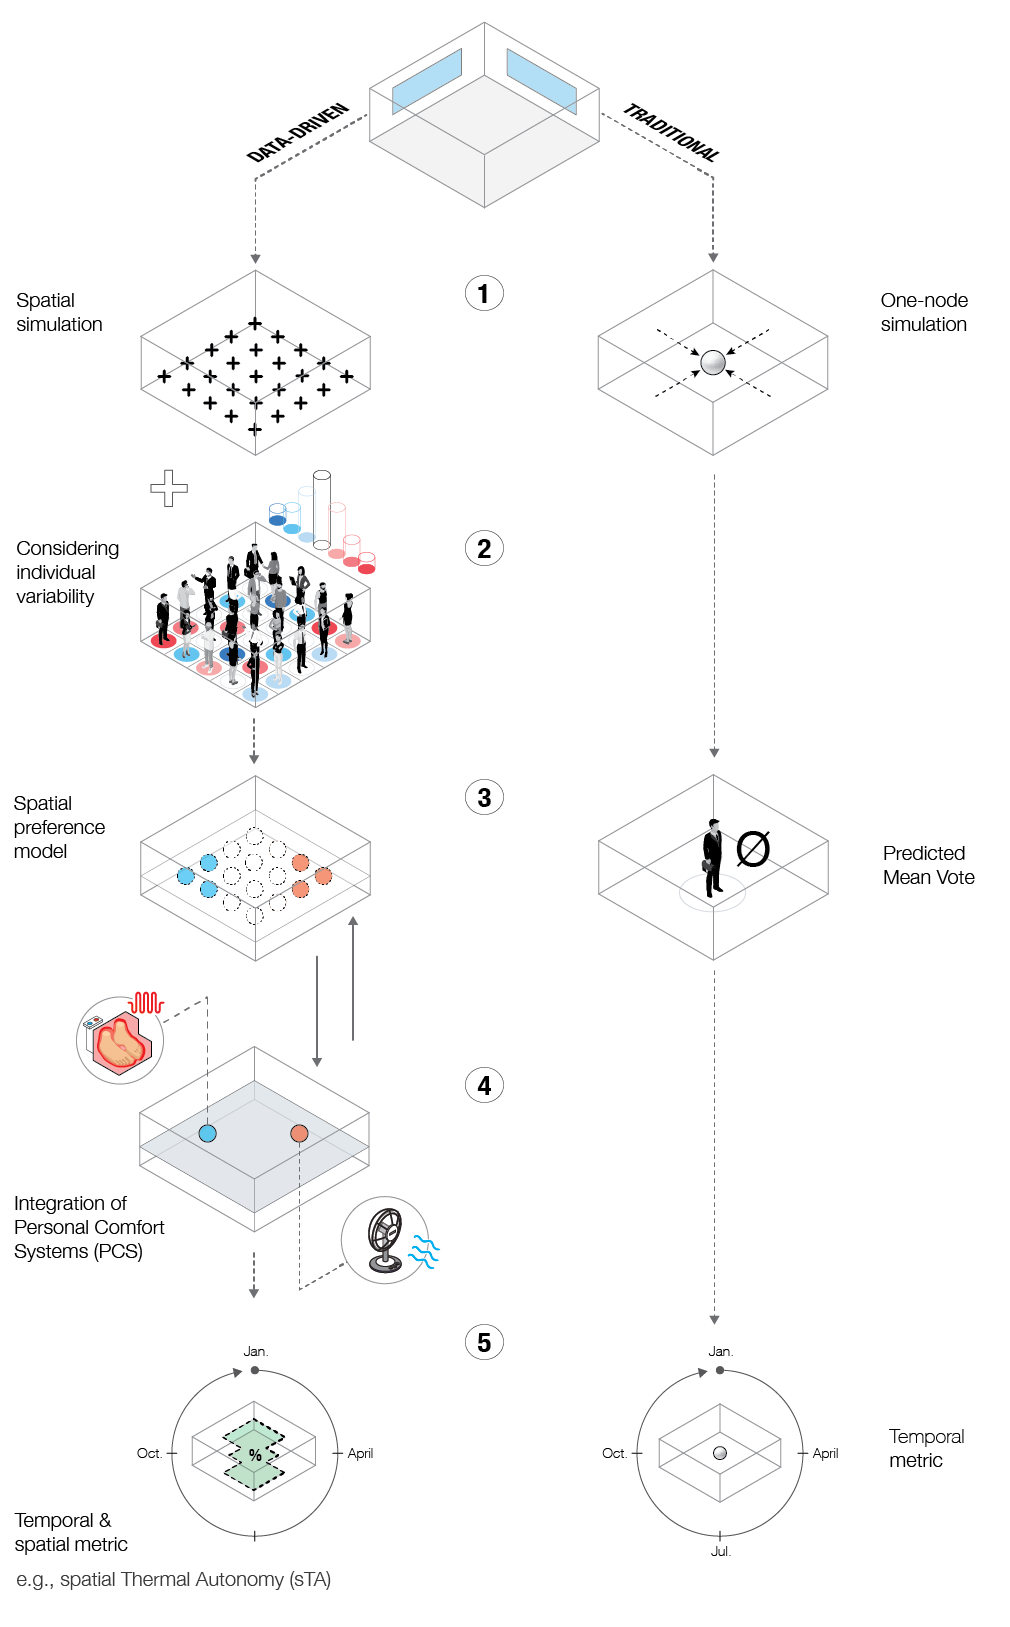
\includegraphics[width=0.9\textwidth]{manuscript/src/figures/workflow-comparison.png}
    \caption{Framework components compared to conventional workflow: Advances in technology and data science enable further development of thermal comfort prediction workflows, including an upgrade of spatial resolution (1), prediction algorithm (3) and metric (5) as well as the inclusion of individual diversity (2) and the impact of Personal Comfort Systems (PCS) (4).}
    \label{fig:framework}
\end{figure}



%%%%%%%%%%%%%%%%%%%%%%%%%%%%%%%%%%%%%%%%%%%%%%

% STRUCTURE FOR ALL PARTS:
% BRIEF PROBLEM REITERATION - SOLUTION - BENEFITS

\subsection{Grid-based analysis}

Buildings have a pronounced spatial thermal heterogeneity \citep{Mishra2016, Clements2019, Kim2019}. Limited computational power made spatially resolved thermal simulations infeasible, but the described technological improvement \citep{Clarke2015} makes it possible to shift to grid-based analyses and allows avoiding the loss of spatial detail when assessing thermal comfort.

Examples of spatially resolved analysis can be found in neighbouring fields in the built environment. \textit{Radiance} \citep{WardRadiance1994} by default generates a grid-based output of high spatial resolution. Although the underlying physical principles in daylight may be more complex and require a more detailed simulation process, the value of spatial output data from these software tools for the building planning process is undisputed. 

For thermal comfort analysis, spatially resolved analysis is of high value. Grid-based simulation outputs shed light on the expected spatial thermal heterogeneity in indoor environmental variables from the early design stages. It is a valuable decision-making tool for modelling thermal comfort and designing conditioning strategies for the building in operation. Regarding \gls{hvac} design, higher simulation detail provides the basis for a shift from centralised, "one-size-fits-all" toward decentralised and more problem-focused solutions for space conditioning.


%%%%%%%%%%%%%%%%%%%%%%%%%%%%%%%%%%%%%%%%%%%%%%

\subsection{Comfort classification}

The low accuracy of conventional thermal comfort models is also attributed to their inability to take personal variability into account \citep{KimSchiavon2018}. Therefore, finding a way to incorporate this diversity would significantly enhance the thermal comfort prediction models.

A promising route is to group the occupants according to their perception of thermal comfort. Previous work has shown that it is feasible to classify occupants into different types of persona \citep{Lee2017, Gauthier2020, Quintana2023}. These clusters can be used as input for thermal comfort models and provide separate predictions for each classification group, reflecting, at least partially, the diversity among building occupants. This would increase awareness and inform the planning of \gls{pcs} and other opportunities for active comfort adaptation in buildings. In turn, this will lead to considerable improvement in occupant comfort and satisfaction by improving flexibility and control.


%%%%%%%%%%%%%%%%%%%%%%%%%%%%%%%%%%%%%%%%%%%%%%

\subsection{Data-driven prediction model}

Conventional thermal comfort indices and their underlying algorithms have two main weaknesses: low accuracy \citep{Cheung2019, Luo2020, KimZhou2018} and they cannot incorporate new information and additional variables into the existing model \citep{VanHoof2008}.

On the contrary, \gls{ml} algorithms allow modelling of complex relationships, are highly versatile and easily integrate new datasets and additional parameters. Several review publications emphasise the successful implementation of \gls{ml} algorithms for the prediction of thermal comfort and highlight their benefits compared to conventional algorithms \citep{KimSchiavon2018, QavidelFard2022}. These include significant improvements in prediction accuracy, high flexibility, and self-learning capability. 

Integrated into a thermal comfort prediction workflow, \gls{ml} models outperform traditional \gls{pmv} and Adaptive algorithms in several ways. Higher prediction accuracy in the building design process may lead to higher levels of thermal comfort during building operation. Moreover, the versatility and improved data handling capability of \gls{ai}-based prediction methods can facilitate the creation of a more effective feedback loop between post-occupancy evaluation data and the implementation of findings into building design. Leveraging these findings, and additional data from other sources within and around the building will lead to dynamic, occupant-centred, and context-specific predictions of thermal comfort during building design and operation.


%%%%%%%%%%%%%%%%%%%%%%%%%%%%%%%%%%%%%%%%%%%%%%

\subsection{PCS integration}

Standard thermal comfort evaluation workflows still do not account for the impact of \gls{pcs} on occupant thermal comfort and building energy use. \gls{pcs} have been shown to improve thermal comfort \citep{Zhang2022}, to increase satisfaction \citep{Kim2019, Zhang2022}, and reduce energy use and overall \gls{hvac} system capacity \citep{Zhang2018, Rawal2020, Knudsen2023}. In addition to these direct benefits of \gls{pcs}, an implementation in \gls{bps} workflows would help to foster individual adaptation and control and further strengthen the validity of passive design solutions, which may not always guarantee comfortable conditions alone.


%%%%%%%%%%%%%%%%%%%%%%%%%%%%%%%%%%%%%%%%%%%%%%

\subsection{Spatial comfort metric}

Conventional thermal comfort metrics used for building design have two major drawbacks (see \Cref{tab:comfort-indices}). They (a) focus on the temporal dimension only, e.g., expected percentage of thermal comfort or discomfort over a year, and (b) disregard, energy-wise, how the envisioned indoor climate is provided.

Adding a spatial dimension to these long-term indices would lead to a more holistic approach that incorporates the spatial thermal diversity of dynamic indoor environments. This is already done in daylighting analysis \citep{Heschong2012, Reinhart2006}. Furthermore, computing the metric without mechanical systems would provide a good measure of the overall design, passive performance, and resilience of the building in the event of a power outage. Building design can be assessed using ventilation, thermal, and luminous autonomy metrics \citep{Ko2018}

\begin{table}[!h]
\centering
\footnotesize
    \caption{Long-term thermal comfort indices in ISO 7730, EN 16798 and ASHRAE 55: All indices included focus on temporal dimension and combine a prediction for hourly thermal simulation results into an annual and single-value metric; spatial dimension is restricted to separation into thermal zones.}
        \label{tab:comfort-indices}
        \renewcommand{\arraystretch}{1.75}
        
            \begin{tabular}{ m{3cm} m{0.75cm} m{0.75cm} m{1.25cm} m{4cm} }

            \textbf{Index} & ISO\newline7730 & EN\newline16798 & ASHRAE\newline55 & \textbf{Limitations} \\
        
            \hline

            Percentage of time outside PMV range & $\bullet$ & $\bullet$ & $\bullet$ & \multirow[t]{2}{4cm}{(i) Measure frequency of discomfort, but not severity; (ii) discontinuous } \\

            % \cline{2-2}

            Percentage of time outside t$_{op}$ range & $\bullet$ & $\bullet$ & $\bullet$ & {} \\

            \hline

            Degree-hours & $\bullet$ & $\bullet$ & {} & {discontinuous} \\

            % \cline{2-2}

            PPD-weighted & $\bullet$ & $\bullet$ & {} & {(i) asymmetric; (ii) discontinuous; (iii) PMV-based} \\

            % \cline{2-2}

            Accumulated PPD & $\bullet$ & {} & {} & {(i) asymmetric; (ii) PMV-based} \\

            \hline

            Average PPD & $\bullet$ & {} & {} & {(i) asymmetric; (ii) PMV-based} \\
            
            \end{tabular}


\end{table}




